\documentclass{article}
\usepackage[utf8]{inputenc}

\title{Advanced Data Structures:\\Exercises}
\author{Constantino Gómez and Cristobal Ortega\\\{name.surname\}@est.fib.upc.edu}
\date{June 2016}

\usepackage{natbib}
\usepackage{graphicx}
\usepackage{listings}
\usepackage{caption}
\usepackage{booktabs}
\usepackage{tabulary}
\usepackage[titletoc]{appendix}
\usepackage{hyperref}
\usepackage{float}
\usepackage[table,xcdraw]{xcolor}
\usepackage{hyphenat}
\hyphenation{Structure Ordered Array balanced insert}

%Use it for listings to not be split when pagebreaks appear
\floatstyle{plain} % optionally change the style of the new float
\newfloat{Code}{H}{myc}
\lstdefinestyle{myC}{
  frame=single,
  captionpos=b,
  belowcaptionskip=1\baselineskip,
  breaklines=true,
  xleftmargin=\parindent,
  morekeywords={nullptr, key},
  language=C++,
  numbers=left,
  numbersep=5pt,
  showstringspaces=false,
  basicstyle=\fontsize{8}{10}\ttfamily,
  keywordstyle=\bfseries\color{blue}\ttfamily,
  commentstyle=\itshape\color{gray}\ttfamily,
  identifierstyle=\color{black},
  stringstyle=\color{red},
}

\newcommand{\tabitem}{~~\llap{\textbullet}~~}


\begin{document}

\maketitle

Exercises from the first part of the course \citep{ads:slides_amalia} about Multidimensional data structures and Metric Data structures

\section{Preliminaries}

\subsection{Make a table showing the pros and cons of data structures}

% Please add the following required packages to your document preamble:
% \usepackage{booktabs}
% \usepackage{graphicx}
% \usepackage[table,xcdraw]{xcolor}
% If you use beamer only pass "xcolor=table" option, i.e. \documentclass[xcolor=table]{beamer}
\begin{table}[H]
	\small
	\centering
    \begin{tabulary}{1.0\textwidth}{L p{0.4\textwidth} p{0.4\textwidth}} 
        \textbf{Data  Structure} & \textbf{\hspace{1cm} Advantages} & \textbf{\hspace{1cm}Disadvantages} \\
        \hline
        \textbf{Array} & \begin{itemize} \item{Quick insertion} \end{itemize} & \begin{itemize} \item{Slow search, deletions} \item{Fixed size} \end{itemize}\\
        
        
        \textbf{Ordered array} & \begin{itemize} \item{Search: O(log n)} \item{Slow insert/delete: O(n)}  \end{itemize} & \begin{itemize} \item{Fixed size} \end{itemize}\\
        
        
        \textbf{Array} & \begin{itemize} \item{Insert/delete fast} \item{Dynamic memory allocation} \item{Almost no extra memory needed} \end{itemize} & \begin{itemize} \item{Insert / delete can be\newline only done in the first element} \item{No search without any auxiliary data structure} \end{itemize}\\
        
        
        \textbf{Queue} & \begin{itemize} \item{Insert/delete fast} \item{Dynamic memory allocation} \item{Almost no extra memory needed} \end{itemize} & \begin{itemize} \item{Insert / delete can be only done in the first element} \item{No search without any auxiliary data structure} \end{itemize}\\
        
        
        \textbf{Linked list} & \begin{itemize} \item{Quick insertion, delete (at the beginning and in the end)} \item{Dynamic memory allocation} \end{itemize} & \begin{itemize} \item{Search O(n)} \item{Needs extra memory for auxiliary variables} \end{itemize}\\
        

    \end{tabulary}
    %\caption{My caption}
    \label{table:data_structs}
\end{table}

\begin{table}[H]
	\small
	\centering
    \begin{tabulary}{1.0\textwidth}{L p{0.4\textwidth} p{0.4\textwidth}} 
        \textbf{Data  Structure} & \textbf{\hspace{5mm} Advantages} & \textbf{\hspace{1cm}Disadvantages} \\
        \hline

        \textbf{BST} & \begin{itemize} \item{Search, insert, delete: O(log n)} \item{Dynamic memory allocation}  \end{itemize} & \begin{itemize} \item{It can be converted to linked list (no balancing)} \item{Needs extra memory for auxiliary variables} \end{itemize}\\
        
        
        \textbf{AVL (BST balanced)} & \begin{itemize} \item{Search, insert, delete: O(log n)} \item{Dynamic memory allocation}  \end{itemize} & \begin{itemize} \item{It has more constant work since every insert /\newline delete  we have to check the level of the children and reorganize the structure if needed} \item{Needs extra memory  for auxiliary variables} \end{itemize}\\
        
        \textbf{Hash table} & \begin{itemize} \item{Average insert / search / delete O(1)} \item{Dynamic memory allocation}  \end{itemize} & \begin{itemize} \item{Worst case O(n)} \item{To keep efficiency changes in the size of the structure may \newline require  to change the hash function} \item{Inefficient for low number of entries} \end{itemize}\\
        
        
        \textbf{Heap} & \begin{itemize} \item{Fixed or dynamic array} \item{Find and insert min O(1) in most cases}  \end{itemize} & \begin{itemize} \item{Partially ordered, search O(n)} \end{itemize}\\
    

    \end{tabulary}
    %\caption{My caption}
    \label{table:data_structs2}
\end{table}


\begin{table}[H]
	\small
	\centering
    \begin{tabulary}{1.0\textwidth}{L p{0.4\textwidth} p{0.4\textwidth}} %{@{}p{0.1\textwidth}p{0.4\textwidth}p{0.4\textwidth}@{}}
        \textbf{Data  Structure} & \textbf{Advantages} & \textbf{Disadvantages} \\
        \hline
        
        \textbf{Heap} & \begin{itemize} \item{Fixed or dynamic array} \item{Find and insert min O(1) in most cases}  \end{itemize} & \begin{itemize} \item{Partially ordered, \newline search O(n)} \end{itemize}\\ 
        
        \textbf{Graph} & \begin{itemize} \item{Abstract datatype, common implementations are: adjacency list, adjacency matrix, and incidence matrix} \end{itemize} & \begin{itemize} \item{Each implementation favors or penalizes a subset of operations: add vertex/edge, remove vertex/edge} \end{itemize}\\
        
    \end{tabulary}
    \caption{Data Structures pros and cons}
    \label{my-label}
\end{table}
\section{Multidimensional Data Structures}

\subsection{Count (give) the number of elements (regions) of the partition of the space
induced by k-d trees of any kind and of k dimensional quad trees.}

\begin{itemize}
    \item Kd-tree
        \begin{itemize}
            \item Cells: \textit{n+1}
            \item Partitions: \textit{n}
        \end{itemize}
    \item Quad-tree
        \begin{itemize}
            \item Cells: \textit{3n+1}
            \item Partitions: \textit{2n}
        \end{itemize}
\end{itemize}

\subsection{Propose a node definition of relaxed k-d trees (in c++) together with the
operations of insertion of a new element, partial match and orthogonal
range searches. How could you implement deletions?}


\begin{lstlisting}[caption=Class Node of relaxed kd-trees, style=myC]
    struct node {
        type Key;
        type discriminant;
        int size;
        node *left, *right;
    };
\end{lstlisting}



\begin{lstlisting}[caption=Insert of relaxed kd-trees, style=myC]
relax_kdtree insert(relax_kdtree t, type& x) {
    if ( t->size == 0)
        type nd = rand(0,dimensions); //not sure
        return insert_at_root(t, x, nd);
    else {
        int d = t->discriminant;
        if (x[d] < t->key[d] )
            t->left = insert(t->left,x)
        else 
            t->right = insert(t->right,x);
    }
    return t;
}
\end{lstlisting}



\begin{lstlisting}[caption=Deletion of relaxed kd-trees, style=myC]
relax_kdtree delete(relax_kdtree t, type& x) {
    //t cannot be empty and has to contain x
    //actually we have to check all the possible coordinates in t->key and x
    if (t->key == x) 
        return delete_node(t)

    int d = t->discriminant;
    if (x[d] < t->key[d])
        t->left = delete(t->left,x)
    else
        t->right = delete(t->right,x)
    return t;
}
\end{lstlisting}



\begin{lstlisting}[caption=Partial match of relaxed kd-trees, style=myC]
//we have some query similar to: (3,*) or (3,2,*)

relax_kdtree partial_match(relax_kdtree t, type& q){
    //t cannot be empty
    //we have to check all the possible coordinates of the key
    if (t->key matches q) 
        results.add(t->key)

    int d = t->discriminant;
    if (d == * ){
        results += partial_match(t->left, q)
        results += partial_match(t->right, q)
        return results;
    }
    if (x[d] < q)
        results += partial_match(t->left,q)
    else
        results += partial_match(t->right,q)

    return results;
}

\end{lstlisting}


\begin{lstlisting}[caption=Orthogonal match of relaxed kd-trees, style=myC]
//we have some query similar to: (3,2)x(radius 1, radius 2), we need to return the points inside that range

relax_kdtree orthogonal_match(relax_kdtree t, type& q){
    //t cannot be empty
    //we have to check all the possible coordinates of the key
    if (t->key matches q) 
        results.add(t->key)

    int d = t->discriminant;
    
    if (x[d] < q) //Check lower bound and upper bounds
        results += partial_match(t->left,q)
    if (x[d] >= q) //Check lower bound and upper bounds
        results += partial_match(t->right,q)

    return results;
}
\end{lstlisting}




\subsection{Propose an experiment to evaluate the average cost of partial match
queries in relaxed k-d trees.}

In the experiment, first we generate randomly a tree. For that we obtain a set of random points, we insert them in the tree.

\begin{lstlisting}[caption=Pseudo-code on how evaluate the average cost of partial match queris in relaxed kd-trees, style=myC]
NUM_EXPLORATIONS = x;

while (num_tests < NUM_EXPLORATIONS)
    size = n;  // number of points
    num_pm = m; // number of partial matches we will try to find in each randomized tree

P = generate_random points(n)

# Create randomized tree
for i in lenght(n):
    T == Null
    insert (T, P[i])

#Create random partial match

//start time accounting
for j = 0; j <  num_pm; j++
pm = generate_partial_match()
partial_match(T, pm) 

//end time accounting

Increase total_time by (Time accounted / number of partial matches (num_pm))
increase num_tests

end while
//Report average total_time of total NUM_EXPLORATIONS

\end{lstlisting}


\subsection{Propose an implementation of k dimensional quad trees (in c++) together
with the operations of insertion of a new element and partial match search.
What can you say about deletions?}

\begin{lstlisting}[caption=Class Node of k dimensional quad trees, style=myC]
struct node{
    int capacity = 2^k;
    Type_k[capacity] key;
    Type_v value;
    node** children[k]; //each of these will contain a subtree for a k dimension
    type points[capacity];
};
\end{lstlisting}



\subsection{Set a recurrence for the average cost of partial match queries in relaxed
k-d trees. Can you solve it?}

\begin{itemize}
    \item In each level of the tree ideally we can follow just one branch (or in the worst case, both)
    \item Each branch we follow it has a cost of log n
    \begin{itemize}
        \item Ideally, we will have to follow only one branch
        \item In the worst case we will have to follow all the branches (the partial match matches all the nodes) that means a cost of n*log n
    \end{itemize}
    \item Then we have: log n $\leq$ average cost $\leq$ n*log n 
\end{itemize}


\subsection{Give an example of a 2-dimensional range tree together with a range query.
Show graphically which are the nodes visited by the search algorithm and
how it performs the search.}

First of all, the algorithm to do a range query in a 2-dimensional range tree is:
\begin{lstlisting}[caption=Algorithm to do a range query, style=myC]
2DRangeQuery([x0,y0]:[x1,y1]) {
    if node is a leaf:
        if range(node) is in range([x0,y0]:[x1,y1])
            return all points that are in the range
        else return NULL
    else
        if discriminant(node) < range([x0,y0]:[x1,y1]) //it depends on which is the discriminant
            return 2DRangeQuery(node->left)
        else if discriminant(node) > range([x0,y0]:[x1,y1])
            return 2DRangeQuey(node->right)
        else
            return 2DRangeQuery(node->left) + 2DRangeQuery(node->right)
}
\end{lstlisting}

For showing demonstration we used the slide we used in the theory class (figure \ref{fig:range_query_example}):

\begin{figure}[H]
  \begin{center}
    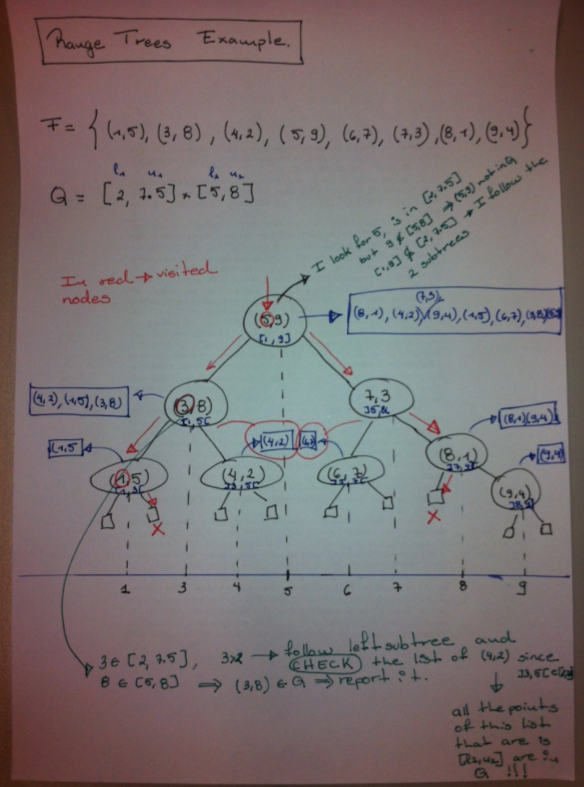
\includegraphics[width=\textwidth]{imgs/range_trees_example.png}
    \caption{Range query example}
    \label{fig:range_query_example}
  \end{center}
\end{figure}

Since we need to traverse the tree in 2 dimensions we spent there log$^2$n (log n if it were just one dimension) and the points we report in the query K.\\
All sum up is: \textit{O(log$^2$n + k)}


\subsection{What is fractional cascading? Give an example in a 2-dimensional range
tree.}

Instead having to traverse all the tree we could have some “sets” that represents each level of our range tree.

\begin{figure}[H]
  \begin{center}
    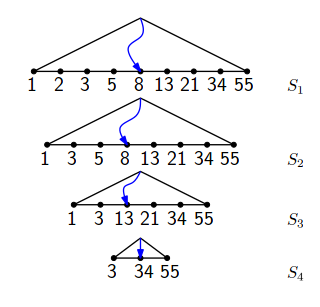
\includegraphics[width=\textwidth]{imgs/fractional_cascading1.png}
    \caption{Sets on a tree}
    \label{fig:fractional_cascading1}
  \end{center}
\end{figure}

Then we just need to find x1 (from [x1,x2] for each Sm and iterate each set until find x2.
But even better, it would be store pointers in each element of S$_{m-1}$ to the smallest element in S$_m$ that is $\leq$ element

\begin{figure}[H]
  \begin{center}
    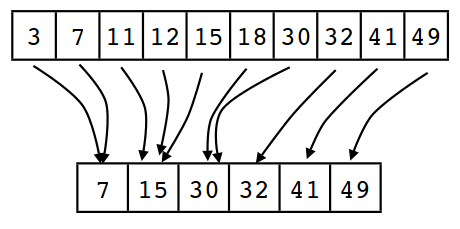
\includegraphics[width=\textwidth]{imgs/fractional_cascading2.png}
    \caption{Pointers for fractional cascading}
    \label{fig:fractional_cascading2}
  \end{center}
\end{figure}

Then, our range search cost will be: \textit{O(log n + k)} \citep{fractional_cascading1}\citep{fractional_cascading2}

\subsection{What are PR (Point region) k-d trees and quad trees?}

K-d trees and quad trees are not divided by a key of each node, instead, the division is made by a fixed criteria and usually a spacial criteria: each node is determined by the coordinates of one point the the space, therefore instead of accessing the trees for a key, it is done by searching for a point.\\
And for the quad-tree the criteria instead of a point, usually it is the center of the region we want to divide: if we have a 2D space that we want to represent it as a quadtree, we would get its center, and divide the space in 4, these 4 would be the children. This also happens in octrees but for 3D spaces.\\

Then, a \textit{Point Region} means the fixed point that we used as a \textit{key} for the node.



\subsection{Show how to represent a 3-D object in a delimited region space using
octrees. Give an example}

If we need to divide a 3D object with an octree, we can get the center of the space containing it (or get the maximum and minimum values of each dimension of the object to use them as container):

\begin{itemize}
    \item The center point (\textit{PR} will be our \textit{key} for our root
    \item Each children will be defined as a sub-space of the space divided for our PR: upper right in the back, upper left in the back, upper right in the front, etc.
\end{itemize}

In the case we want to have a maximum of points per children, we can apply it recursively.

One example is illustrated in figure \ref{fig:octree_example}

\begin{figure}[H]
  \begin{center}
    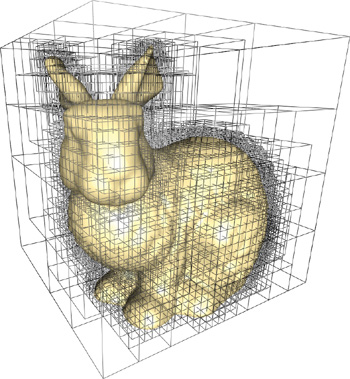
\includegraphics{imgs/octree_example.jpg}
    \caption{An object contained in octrees}
    \label{fig:octree_example}
  \end{center}
\end{figure}

\newpage

\section{Metric Data Structures}
\subsection{Discuss the dynamism of the data structures presented in this topic.}
This kind of data structure are used to do different searches: 

\begin{itemize}
    \item Range queries
    \item Nearest neighbor queries
    \item k-Nearest neighbor queries
\end{itemize}

And in a \textit{general} data structure these queries are usually resolved with brute force (checking each point against all the others); this is too costly. To be able to do such queries efficiently, we need metric data structures.\\
\\
The problem in these metric data structures comes with insertions and deletions. These data structures are usually built once and \textit{queried} enough times to payback the built cost; while permitting efficient insertions is quite usual, deletions are rarely handled. In several indexes one can delete some elements, but there are selected elements that cannot be delete at all, in that situation, deleting an element could require to scrap and rebuild the data structure. \citep{dynamism}

\subsection{What are approximate nearest neighbor queries? Look for a data structure that deals with them, describe it and give its properties.}

Nearest neighbor $query NN(q)$: retrieve from U the closest element to q:\\
$NN(q) = { u \in U | d(u,q) \leq d(v,q) \forall v \in U}$

An example would be: Geometric Near-neighbor Access Tree (GNAT)
It is based on the philosophy that the data structure should act as a hierarchical geometrical model of the data as opposed to a simple decomposition of the data which does not use its intrinsic geometry.

The offered performance can be seen in table \ref{table:gnat}, where n is the number of nodes (non empty) and k is the average degree (equal to N/n). As the tables specifies, the author of the data structure have been not able to determine a domain or boundaries for the query time. \citep{GNAT}

\begin{table}[H]
    \centering
    \begin{tabular}{cc}
    \hline
    Characteristic & Cost           \\ \hline
    Space          & O($n_m$ + N)      \\
    Build          & O($N_m \times log (m)\times N$ \\
    Query time     & Not analyzed   \\ \hline
    \end{tabular}
    \caption{GNAT characteristics}
    \label{table:gnat}
\end{table}


\bibliographystyle{plain}
\bibliography{references}
\end{document}
